\begin{figure}
\begin{center}

\begin{subfigure}[b]{\columnwidth}
\centering
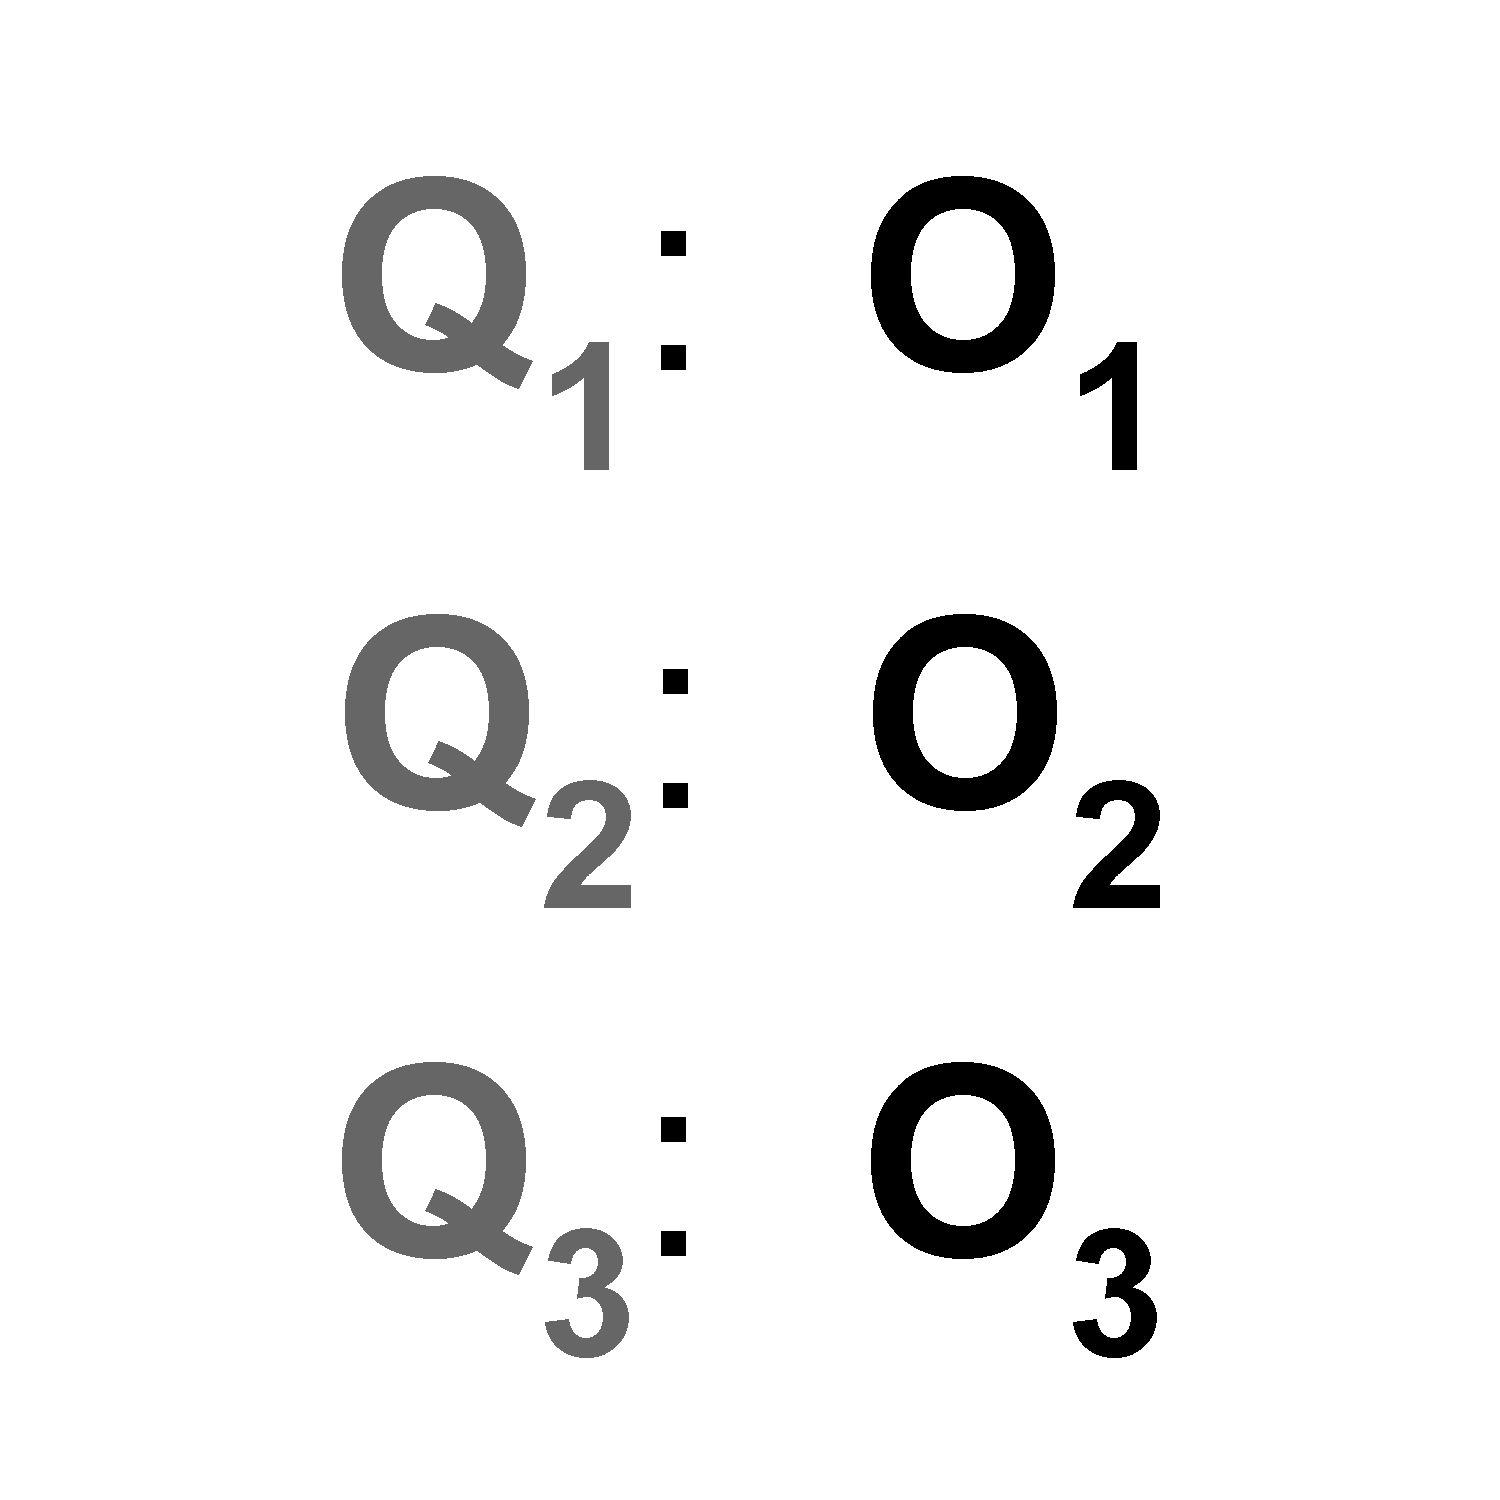
\includegraphics[width=0.33\columnwidth]{img/1d-2d-single-double/single}%
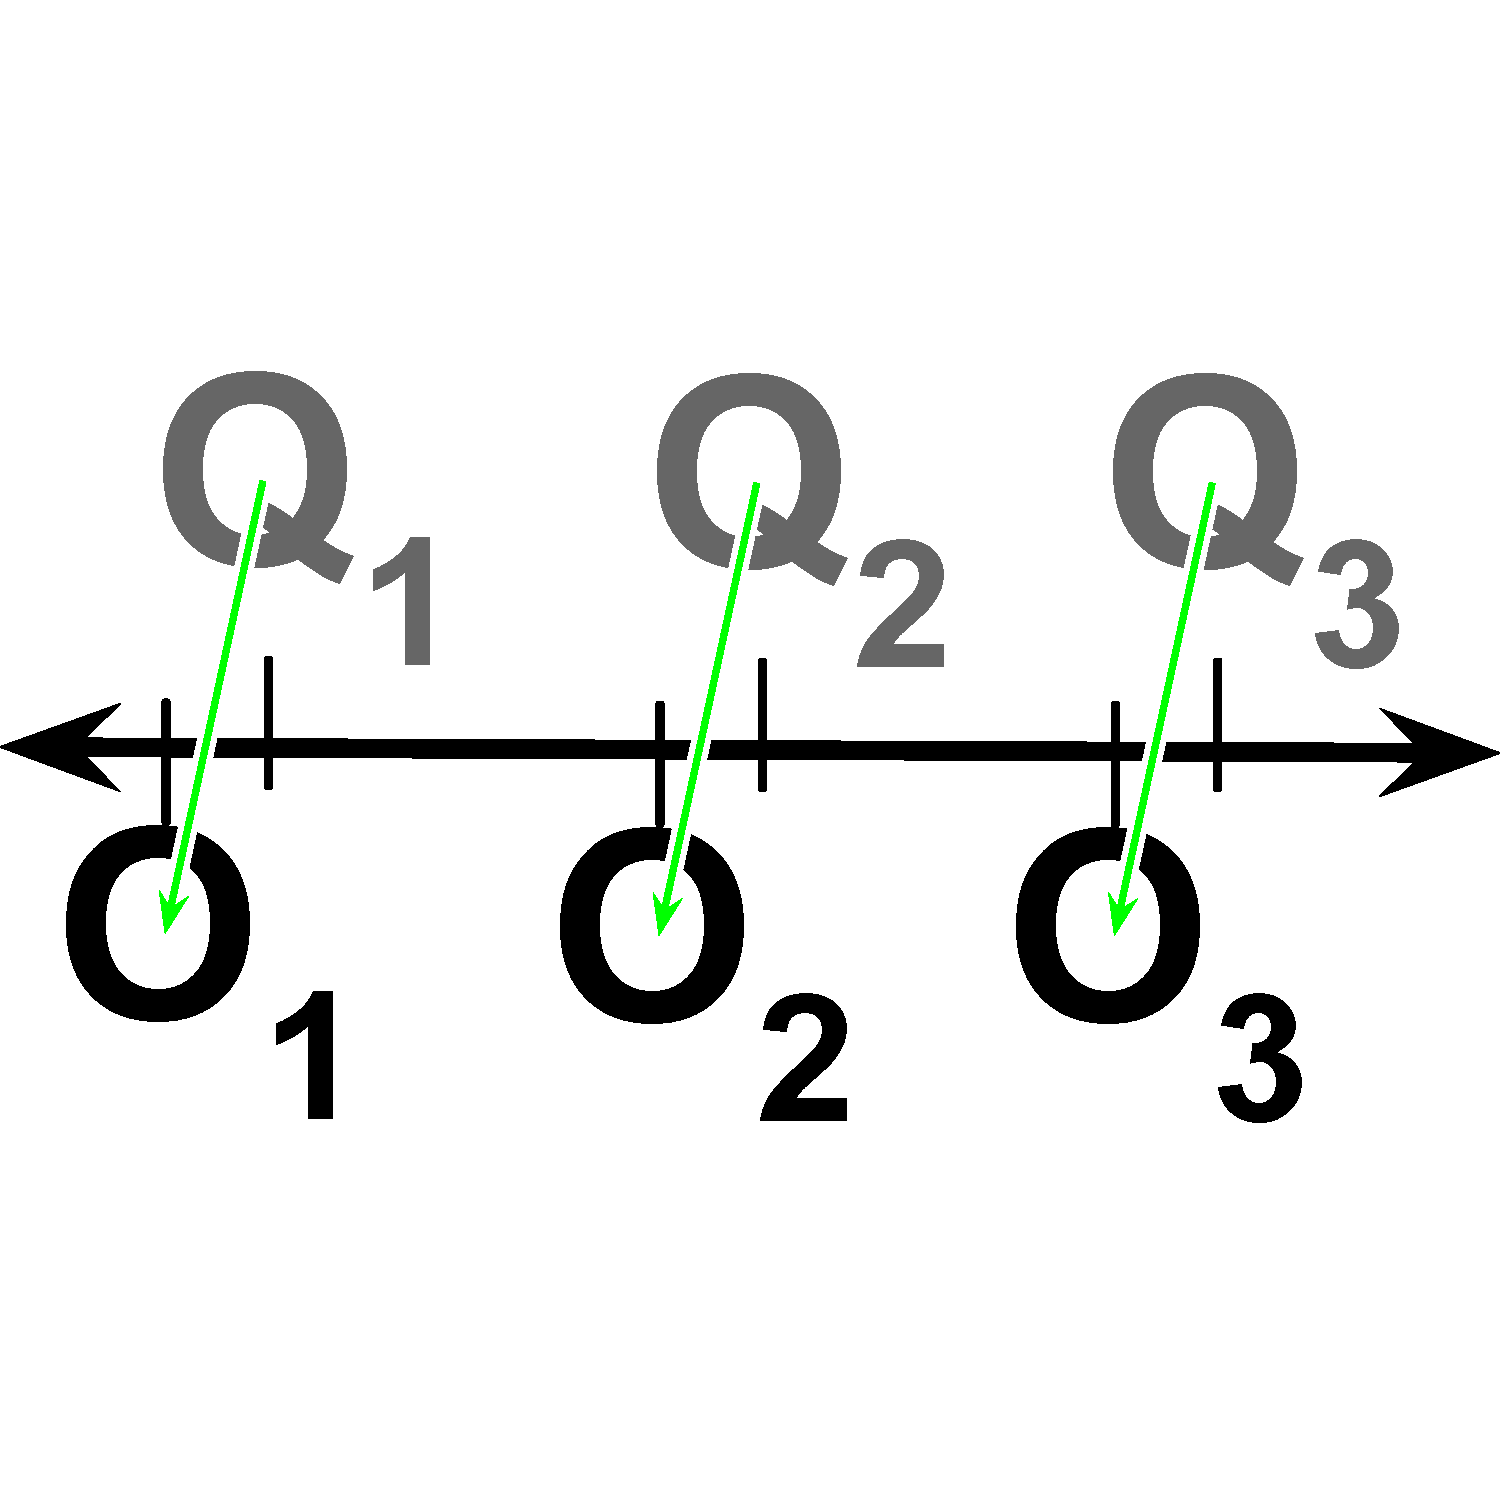
\includegraphics[width=0.33\columnwidth]{img/1d-2d-single-double/1d-single}%
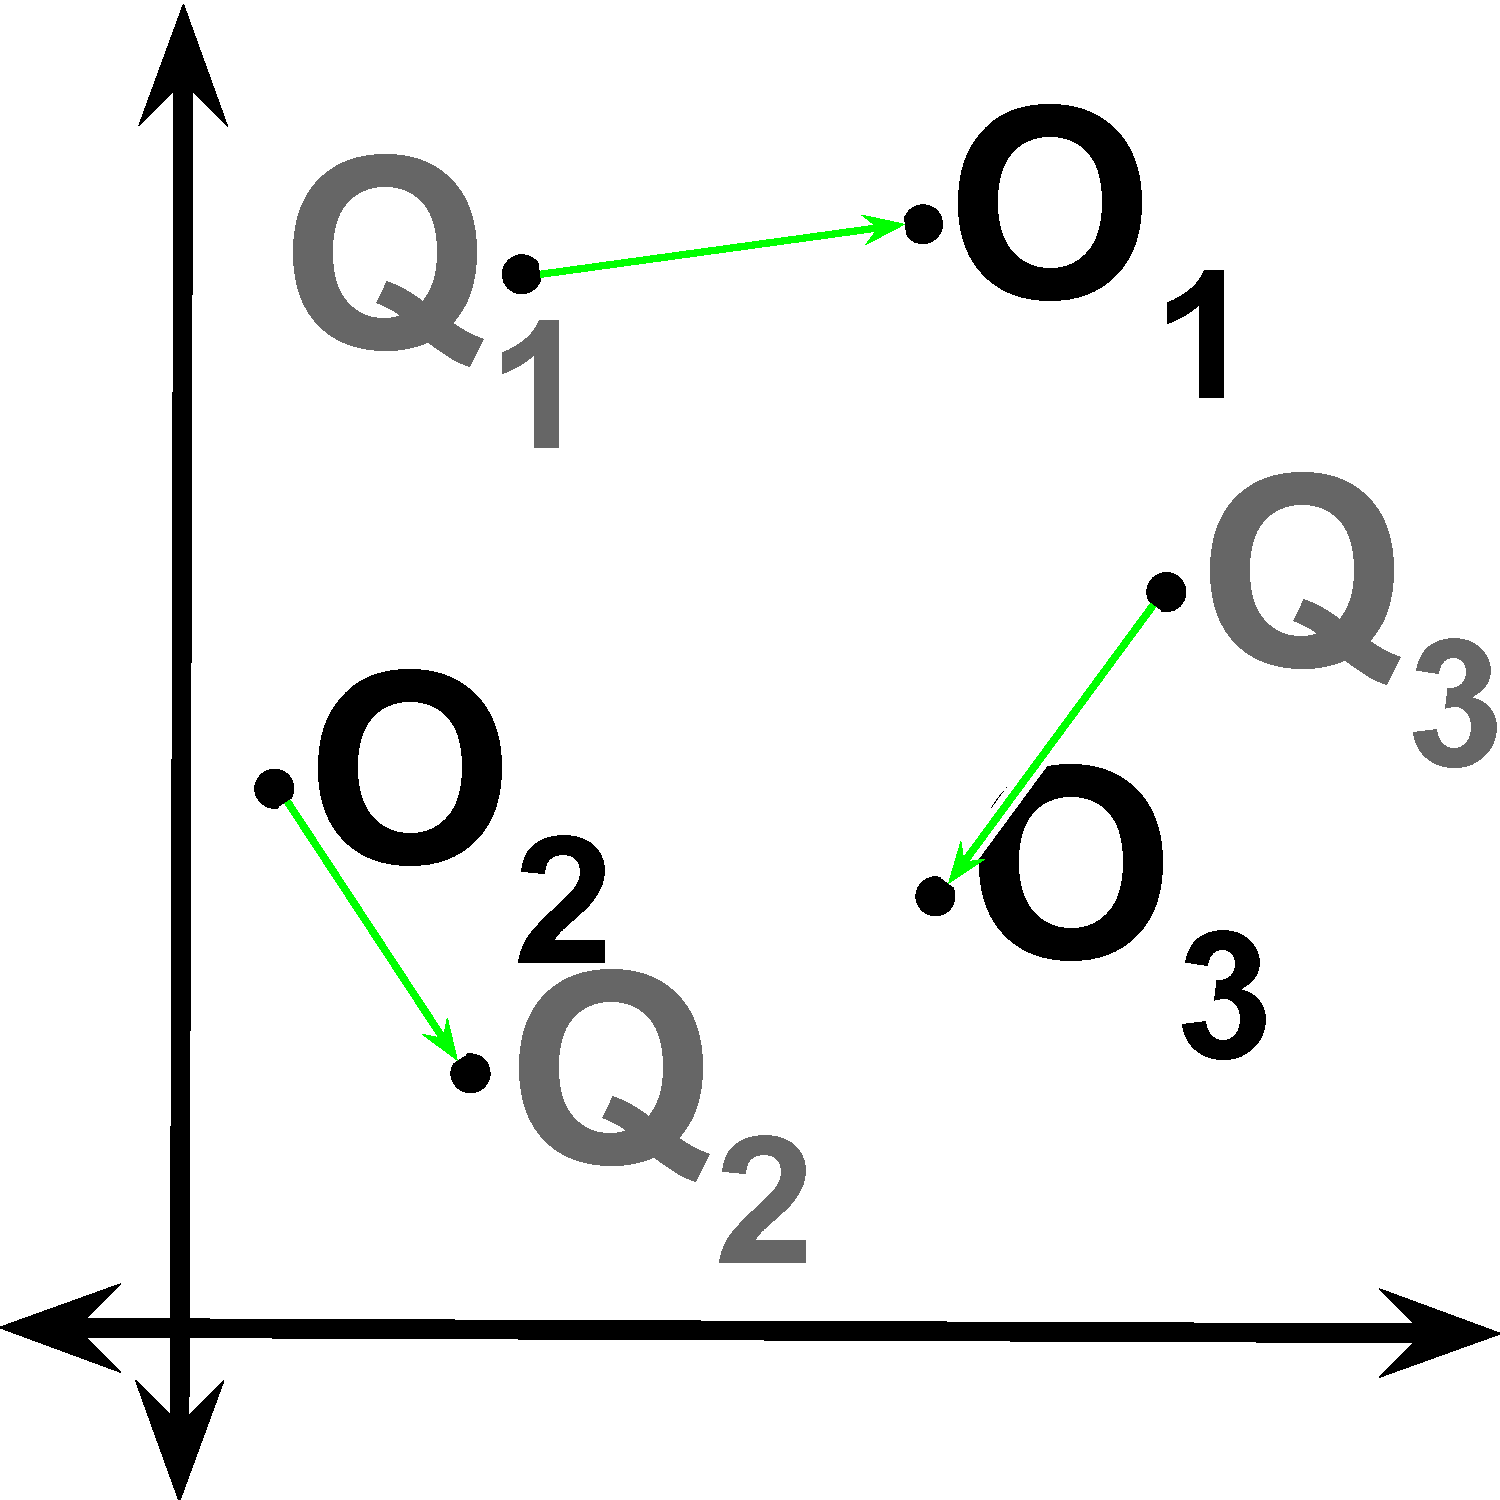
\includegraphics[width=0.33\columnwidth]{img/1d-2d-single-double/2d-single}
\caption{
Single-operand matching constraint
}
\label{fig:single}
\end{subfigure}

\begin{subfigure}[b]{\columnwidth}
\centering
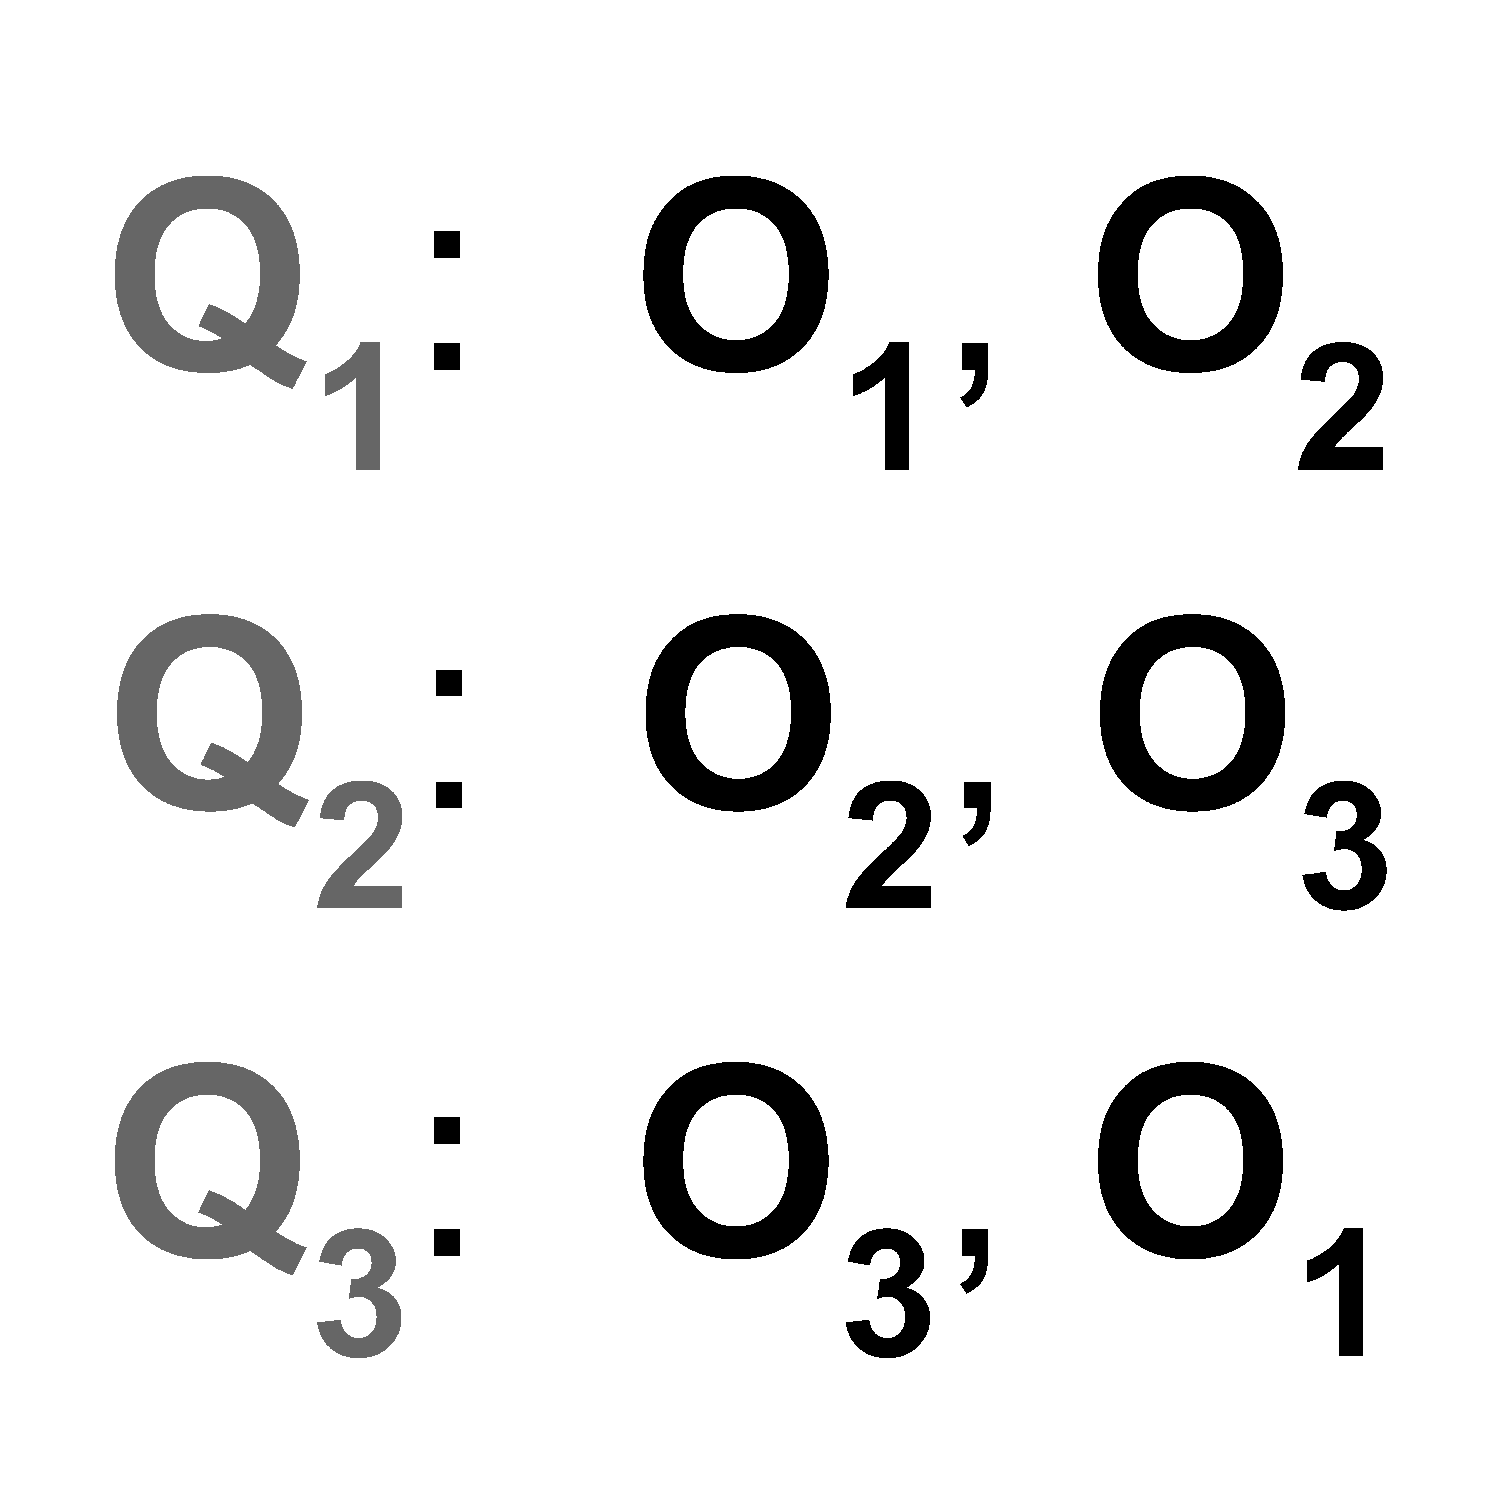
\includegraphics[width=0.33\columnwidth]{img/1d-2d-single-double/double}%
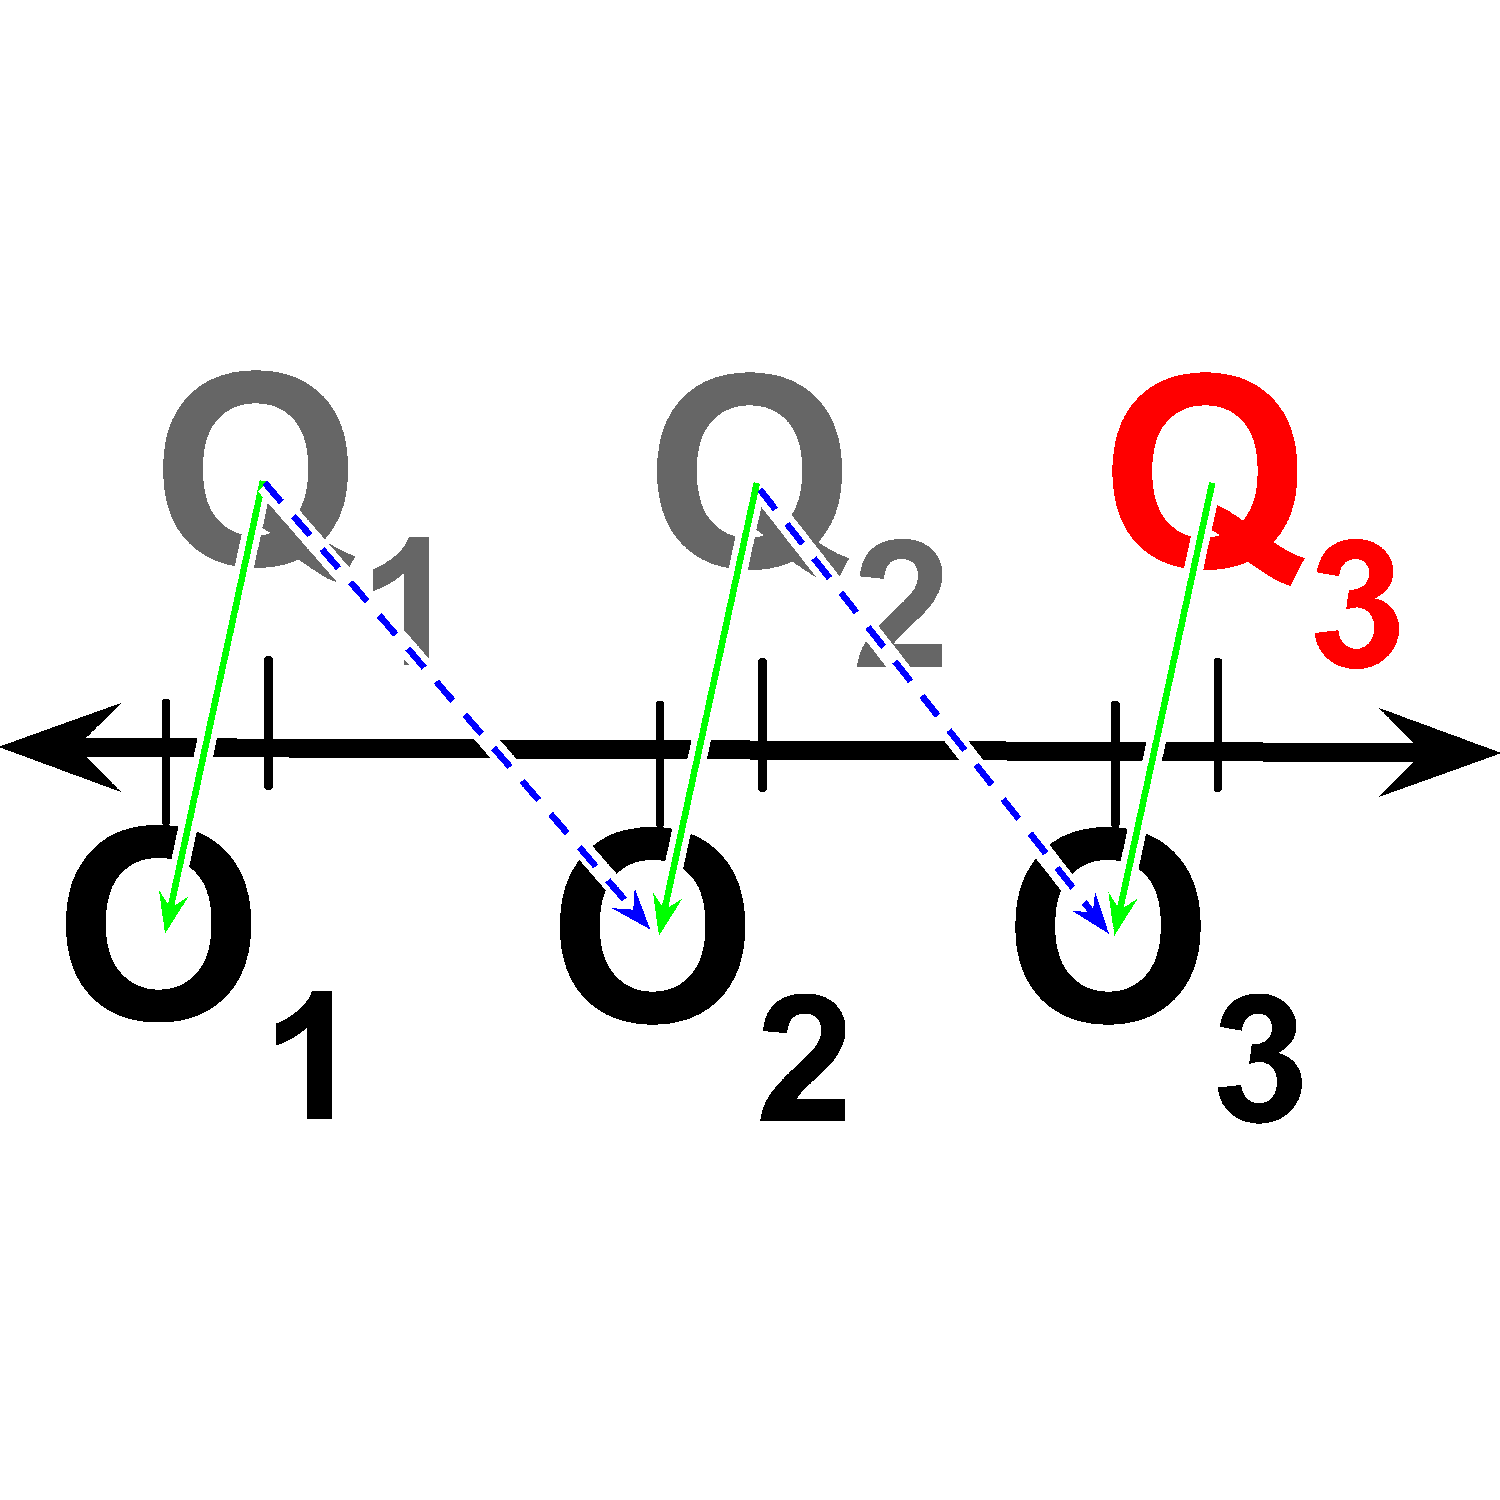
\includegraphics[width=0.33\columnwidth]{img/1d-2d-single-double/1d-double}%
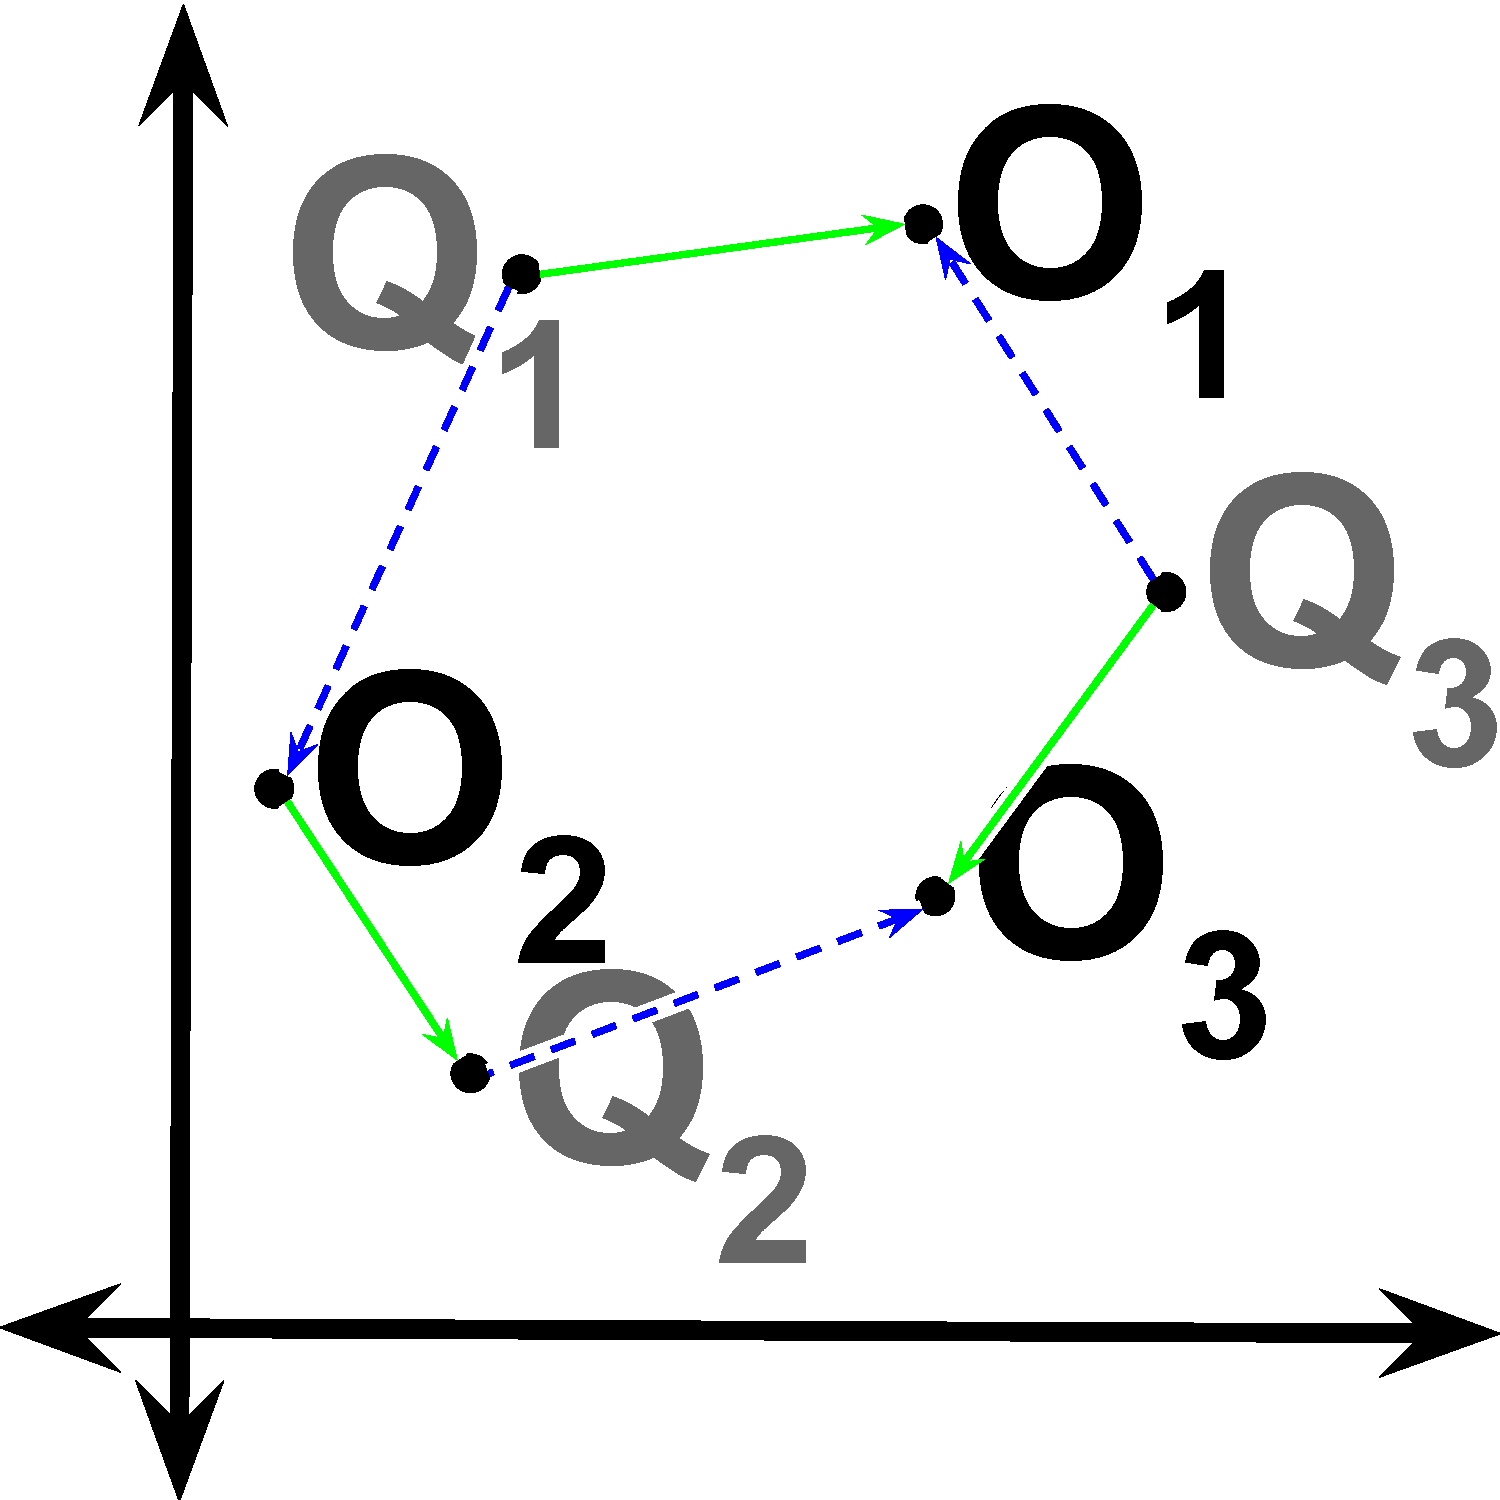
\includegraphics[width=0.33\columnwidth]{img/1d-2d-single-double/2d-double}
\caption{
Double-operand matching constraint
}
\label{fig:double}
\end{subfigure}

\caption{
A cartoon depicting the necessity of tag space dimensionality to satisfy multi-operand matching constraints.
}
\label{fig:1d_2d_single_double}

\end{center}
\end{figure}
